
\begin{frame}{Cavità 2D}

  \begin{figure}
     \fbox{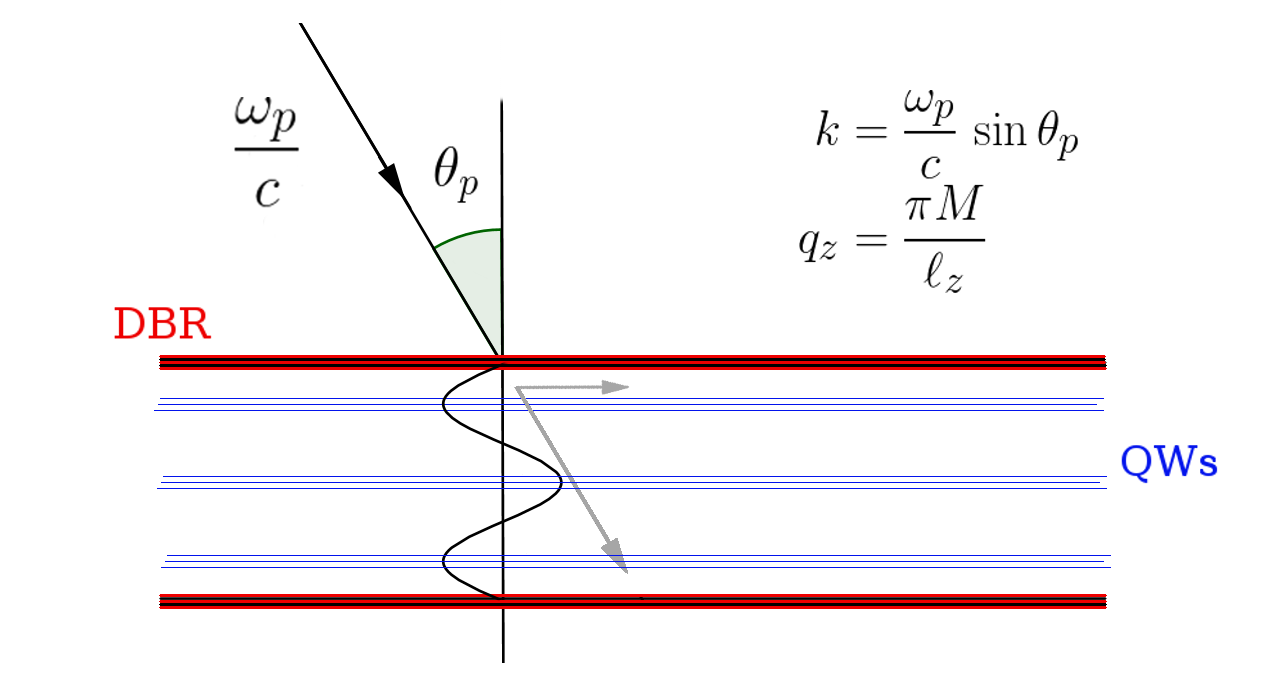
\includegraphics[height=.4\textheight]{pics/QW_field.png}}
    \end{figure}

    Massa del fotone dipendente dallo stato trasverso eccitato

    \begin{columns}
     \begin{column}{.5\textwidth}
      \begin{align*}
        \omega_C(k) &= \frac{c}{n_0}\sqrt{{q_z}^2 + k^2} \\
                &\simeq \omega_C^0 + \frac{\hbar k^2}{2m_C} &&
        \end{align*}
     \end{column}

     \begin{column}{.6\textwidth}
      \begin{figure}
       \fbox{
       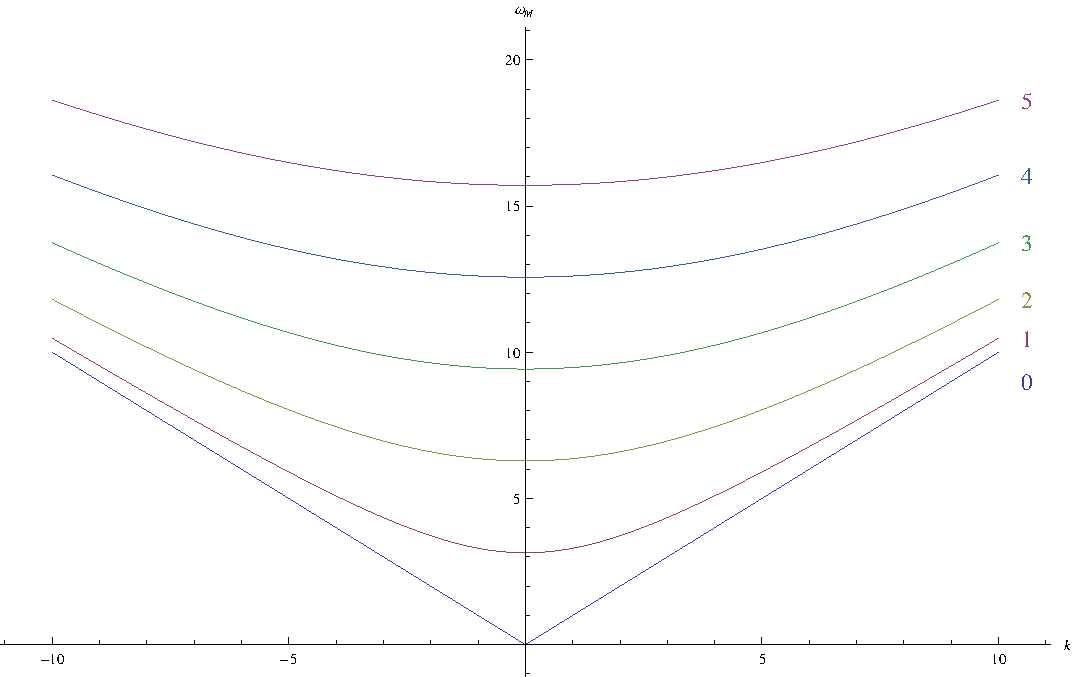
\includegraphics[width=.7\columnwidth]{pics/Photon_dispersion.pdf}}
      \end{figure}

     \end{column}


    \end{columns}


        
\end{frame}

 \begin{frame}{Quantum Wells}
 \alert{DA UNIRE A QUELLA SOPRA}

 Buche/elettroni confinati lungo z \( \longrightarrow \) Eccitoni\\
 \vspace{10pt}
 Si comportano come bosoni\\
 Interagiscono con il campo laser nella cavità

 \begin{flalign*}
 \qquad &\omega_X(k) = \omega_X^0 + \frac{\hbar k^2}{2m_X} \\
  &V_{dip} \propto \vec d_X \cdot \vec E_{cav}
  &&
 \end{flalign*}
  \begin{figure}
  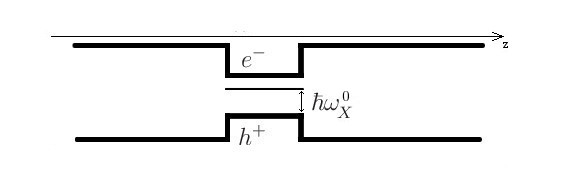
\includegraphics[width=\textwidth]{pics/QW.jpg}
 \end{figure}
   \end{frame}

\subsection{Dinamica dei polaritoni}
 
\begin{frame}{Polaritoni}


  Gradi di libertà sul piano $xy$
  \begin{itemize}
    \item fotoni della cavità
    \item eccitoni, con interaz. di dipolo \(\big(\Omega_R \ll \omega_C, \omega_X \rightarrow \text{RWA}\big)\)
  \end{itemize}

  
 \begin{equation*}
 \boxed{
     \ham_{free} = \hbar \displaystyle \intk
      \begin{pmatrix} \oa_C^\dagger & \oa_X^\dagger \end{pmatrix}\,
      \begin{pmatrix} \omega_C & \Omega_R \\ \Omega_R & \omega_X \end{pmatrix}\,\begin{pmatrix}\oa_C \\ \oa_X \end{pmatrix}
    }  
   \end{equation*}

% \begin{equation*}
% %\begin{align}
%  \ham_{free} = \hbar \intk \omega_{LP} (k) \oa_{LP}^\dagger \oa_{LP} ~ + ~ \omega_{UP} (k) \oa_{UP}^\dagger \oa_{UP}
% %\end{align}
% \end{equation*}
\vspace{-15pt}
\begin{minipage}{\textwidth}
\begin{columns}
\hskip.4cm
\footnotesize{
  \begin{column}{.45\textwidth}
   \begin{flalign*}
    \begin{cases}
        \oa_C = C\lp \ \oa\lp + C\up \ \oa\up \\
        \oa_X = X\lp \ \oa\lp + X\up \ \oa\up
     \end{cases}
     &&
   \end{flalign*}


   Coefficienti di Hopfield\\
   {\scriptsize \(\big( C_j (k) \approx X_j (k) \approx 1/2 \quad \text{@low }k\big)\)}

   \begin{equation*}
    \begin{align}
      &\displaystyle\omega_{ {\scriptstyle (UP,LP)} } (k) = \frac{\omega_C (k) + \omega_X (k)}{2} \\
                             &\pm \left[\Omega_R^2 + \left(\frac{\omega_C (k) - \omega_X (k)}{2}\right)^2\right]^{1/2}
    \end{align}
   \end{equation*}
   Dispersione
    \end{column}
  }
  \hfill
  \begin{column}{.55\textwidth}
   \begin{figure}[h]
    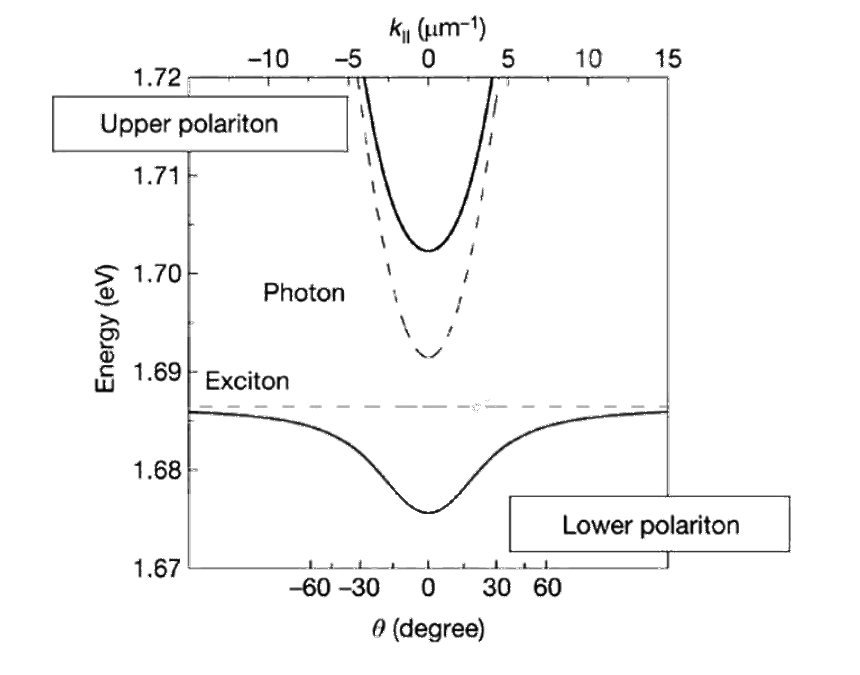
\includegraphics[scale=.2]{pics/polariton_dispersion.png}
   \end{figure}

  \end{column}
\end{columns}
\end{minipage}

\end{frame}



\subsection{Interazioni}

\begin{frame}{Interazioni}
  %\transwipe[direction=270]
  Di carattere fotonico ed elettronico\\
  \footnotesize
  (le ultime sono dominanti)
  \normalsize
  \vskip.5cm
  \begin{itemize}
   \item {
   Nonlinearità ottiche
          \begin{flalign*}
           \chi^{(3)}{\vec E_{cav}}^4 \propto \chi^{(3)}(\oa_C^\dagger + \oa_C)^4 &&
          \end{flalign*}
   }
   \item{
   Scattering coulombiano tra eccitoni
            \begin{flalign*}
             \text{\large{$\tilde V$}} (k,k',q) \ \oa_X^\dagger (k+q) \oa_X^\dagger (k'-q) \oa_X (k') \oa_X (k) &&
            \end{flalign*}
   }
  \end{itemize}

  %\pause
        
\begin{columns}
 \begin{column}
  {.8\textwidth}
  \begin{equation*}
    \boxed{
      \ham_{int} = \intr \sum_{j=X,C} \frac{\hbar g_j}{2} \ \opsi_j^\dagger (r) \opsi_j^\dagger (r) \opsi_j (r) \opsi_j (r)
        }
   \end{equation*}
 \end{column}
  \begin{column}
  {.2\textwidth}
  \begin{itemize}
   \item $ka \ll 1$
   \item RWA
  \end{itemize}

 \end{column}


\end{columns}

\end{frame}

\subsection{Pumping \& losses}

\begin{frame}{Pompaggio laser}
  \begin{columns}
 \begin{column}{.5\textwidth}
    \begin{figure}
         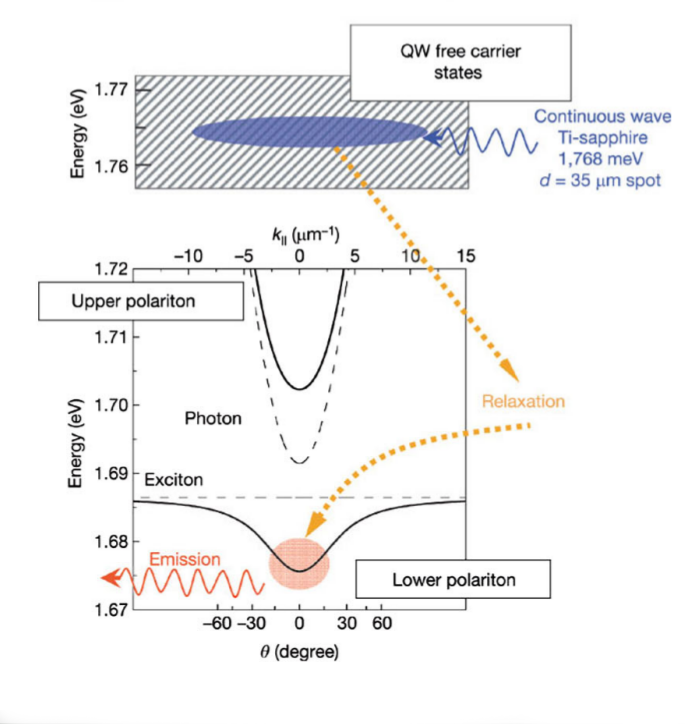
\includegraphics[width=\columnwidth]{pics/incoherent.png}
    \end{figure}

 \end{column}
  \begin{column}{.5\textwidth}
\footnotesize
     \textbf{Non coerente}\\
    % Alto detunig; Rilassamento; Altro...\\
     Fase del modo LP non fissata\\
    % Signal-idler condensate
     \vskip15pt
     \textbf{Coerente}\\
     Fase del condensato fissata dal laser\\
     si può includere nella dinamica
   \end{column}
\end{columns}

 \begin{equation*}
 \boxed{
    \begin{align*}
       \ham_{pump} &=\intr i\hbar \ \eta E_{inc} \ e^{ik_p r -i\omega_p t} \ \opsi_C^\dagger (r) +\hc \\
        &= \quad i\hbar \ \eta E_{inc} \ e^{-i\omega_p t} \ \oa_C^\dagger (k_p) +\hc
    \end{align*}
    }
 \end{equation*}
\end{frame}

\begin{frame}{Dissipazione}
Dovuta all'emissione attraverso gli specchi (trasmittività $\neq 0$)\\
smorzamento radiativo descritto con una master equation
%{\Large
\begin{equation*}
i\hbar \partial_t\ \rho = [\ham,\rho] + i\hbar \lind \rho
\end{equation*}
%}
con operatore di Lindblad 
\begin{flalign*}
\lind \rho = \intk \frac{\gamma_{{\scriptscriptstyle rad}}}{2} \left ( 2\oa_C\rho \oa_C^\dagger - \oa_C^\dagger \oa_C \rho - \rho \oa_C^\dagger \oa_C \right ) &&
\end{flalign*}
$\Rightarrow$ Ha l'effetto di inserire nell'equazione di Heisemberg per $\opsi_C$ un termine di smorzamento:
\[
 i \partial_t\, \opsi_C = \dots -i\frac{\gamma_{{\scriptscriptstyle rad}}}{2} \opsi_C
\]

% \begin{figure}
%        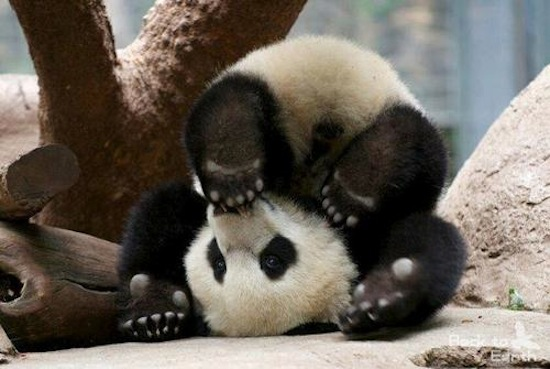
\includegraphics[scale=.3]{pics/Panda.jpg}
%        \caption{\footnotesize Qui ci rimetto il panda, che almeno lui mi fa compagnia}
%       \end{figure}

\end{frame}


